\documentclass[twoside]{book}

% Packages required by doxygen
\usepackage{fixltx2e}
\usepackage{calc}
\usepackage{doxygen}
\usepackage[export]{adjustbox} % also loads graphicx
\usepackage{graphicx}
\usepackage[utf8]{inputenc}
\usepackage{makeidx}
\usepackage{multicol}
\usepackage{multirow}
\PassOptionsToPackage{warn}{textcomp}
\usepackage{textcomp}
\usepackage[nointegrals]{wasysym}
\usepackage[table]{xcolor}

% Font selection
\usepackage[T1]{fontenc}
\usepackage[scaled=.90]{helvet}
\usepackage{courier}
\usepackage{amssymb}
\usepackage{sectsty}
\renewcommand{\familydefault}{\sfdefault}
\allsectionsfont{%
  \fontseries{bc}\selectfont%
  \color{darkgray}%
}
\renewcommand{\DoxyLabelFont}{%
  \fontseries{bc}\selectfont%
  \color{darkgray}%
}
\newcommand{\+}{\discretionary{\mbox{\scriptsize$\hookleftarrow$}}{}{}}

% Page & text layout
\usepackage{geometry}
\geometry{%
  a4paper,%
  top=2.5cm,%
  bottom=2.5cm,%
  left=2.5cm,%
  right=2.5cm%
}
\tolerance=750
\hfuzz=15pt
\hbadness=750
\setlength{\emergencystretch}{15pt}
\setlength{\parindent}{0cm}
\setlength{\parskip}{0.2cm}
\makeatletter
\renewcommand{\paragraph}{%
  \@startsection{paragraph}{4}{0ex}{-1.0ex}{1.0ex}{%
    \normalfont\normalsize\bfseries\SS@parafont%
  }%
}
\renewcommand{\subparagraph}{%
  \@startsection{subparagraph}{5}{0ex}{-1.0ex}{1.0ex}{%
    \normalfont\normalsize\bfseries\SS@subparafont%
  }%
}
\makeatother

% Headers & footers
\usepackage{fancyhdr}
\pagestyle{fancyplain}
\fancyhead[LE]{\fancyplain{}{\bfseries\thepage}}
\fancyhead[CE]{\fancyplain{}{}}
\fancyhead[RE]{\fancyplain{}{\bfseries\leftmark}}
\fancyhead[LO]{\fancyplain{}{\bfseries\rightmark}}
\fancyhead[CO]{\fancyplain{}{}}
\fancyhead[RO]{\fancyplain{}{\bfseries\thepage}}
\fancyfoot[LE]{\fancyplain{}{}}
\fancyfoot[CE]{\fancyplain{}{}}
\fancyfoot[RE]{\fancyplain{}{\bfseries\scriptsize Generated on Sun Mar 22 2015 16\+:36\+:21 for Test by Doxygen }}
\fancyfoot[LO]{\fancyplain{}{\bfseries\scriptsize Generated on Sun Mar 22 2015 16\+:36\+:21 for Test by Doxygen }}
\fancyfoot[CO]{\fancyplain{}{}}
\fancyfoot[RO]{\fancyplain{}{}}
\renewcommand{\footrulewidth}{0.4pt}
\renewcommand{\chaptermark}[1]{%
  \markboth{#1}{}%
}
\renewcommand{\sectionmark}[1]{%
  \markright{\thesection\ #1}%
}

% Indices & bibliography
\usepackage{natbib}
\usepackage[titles]{tocloft}
\setcounter{tocdepth}{3}
\setcounter{secnumdepth}{5}
\makeindex

% Hyperlinks (required, but should be loaded last)
\usepackage{ifpdf}
\ifpdf
  \usepackage[pdftex,pagebackref=true]{hyperref}
\else
  \usepackage[ps2pdf,pagebackref=true]{hyperref}
\fi
\hypersetup{%
  colorlinks=true,%
  linkcolor=blue,%
  citecolor=blue,%
  unicode%
}

% Custom commands
\newcommand{\clearemptydoublepage}{%
  \newpage{\pagestyle{empty}\cleardoublepage}%
}


%===== C O N T E N T S =====

\begin{document}

% Titlepage & ToC
\hypersetup{pageanchor=false,
             bookmarks=true,
             bookmarksnumbered=true,
             pdfencoding=unicode
            }
\pagenumbering{roman}
\begin{titlepage}
\vspace*{7cm}
\begin{center}%
{\Large Test }\\
\vspace*{1cm}
{\large Generated by Doxygen 1.8.9.1}\\
\vspace*{0.5cm}
{\small Sun Mar 22 2015 16:36:21}\\
\end{center}
\end{titlepage}
\clearemptydoublepage
\tableofcontents
\clearemptydoublepage
\pagenumbering{arabic}
\hypersetup{pageanchor=true}

%--- Begin generated contents ---
\chapter{Hierarchical Index}
\section{Class Hierarchy}
This inheritance list is sorted roughly, but not completely, alphabetically\+:\begin{DoxyCompactList}
\item Test2\begin{DoxyCompactList}
\item \contentsline{section}{Test}{\pageref{class_test}}{}
\end{DoxyCompactList}
\end{DoxyCompactList}

\chapter{Data Structure Index}
\section{Data Structures}
Here are the data structures with brief descriptions\+:\begin{DoxyCompactList}
\item\contentsline{section}{\hyperlink{class_test}{Test} \\*Brief description }{\pageref{class_test}}{}
\end{DoxyCompactList}

\chapter{File Index}
\section{File List}
Here is a list of all documented files with brief descriptions\+:\begin{DoxyCompactList}
\item\contentsline{section}{\hyperlink{test_8js}{test.\+js} \\*File for \hyperlink{class_test}{Test} function }{\pageref{test_8js}}{}
\end{DoxyCompactList}

\chapter{Data Structure Documentation}
\hypertarget{class_test}{}\section{Test Class Reference}
\label{class_test}\index{Test@{Test}}


Brief description.  


Inheritance diagram for Test\+:\begin{figure}[H]
\begin{center}
\leavevmode
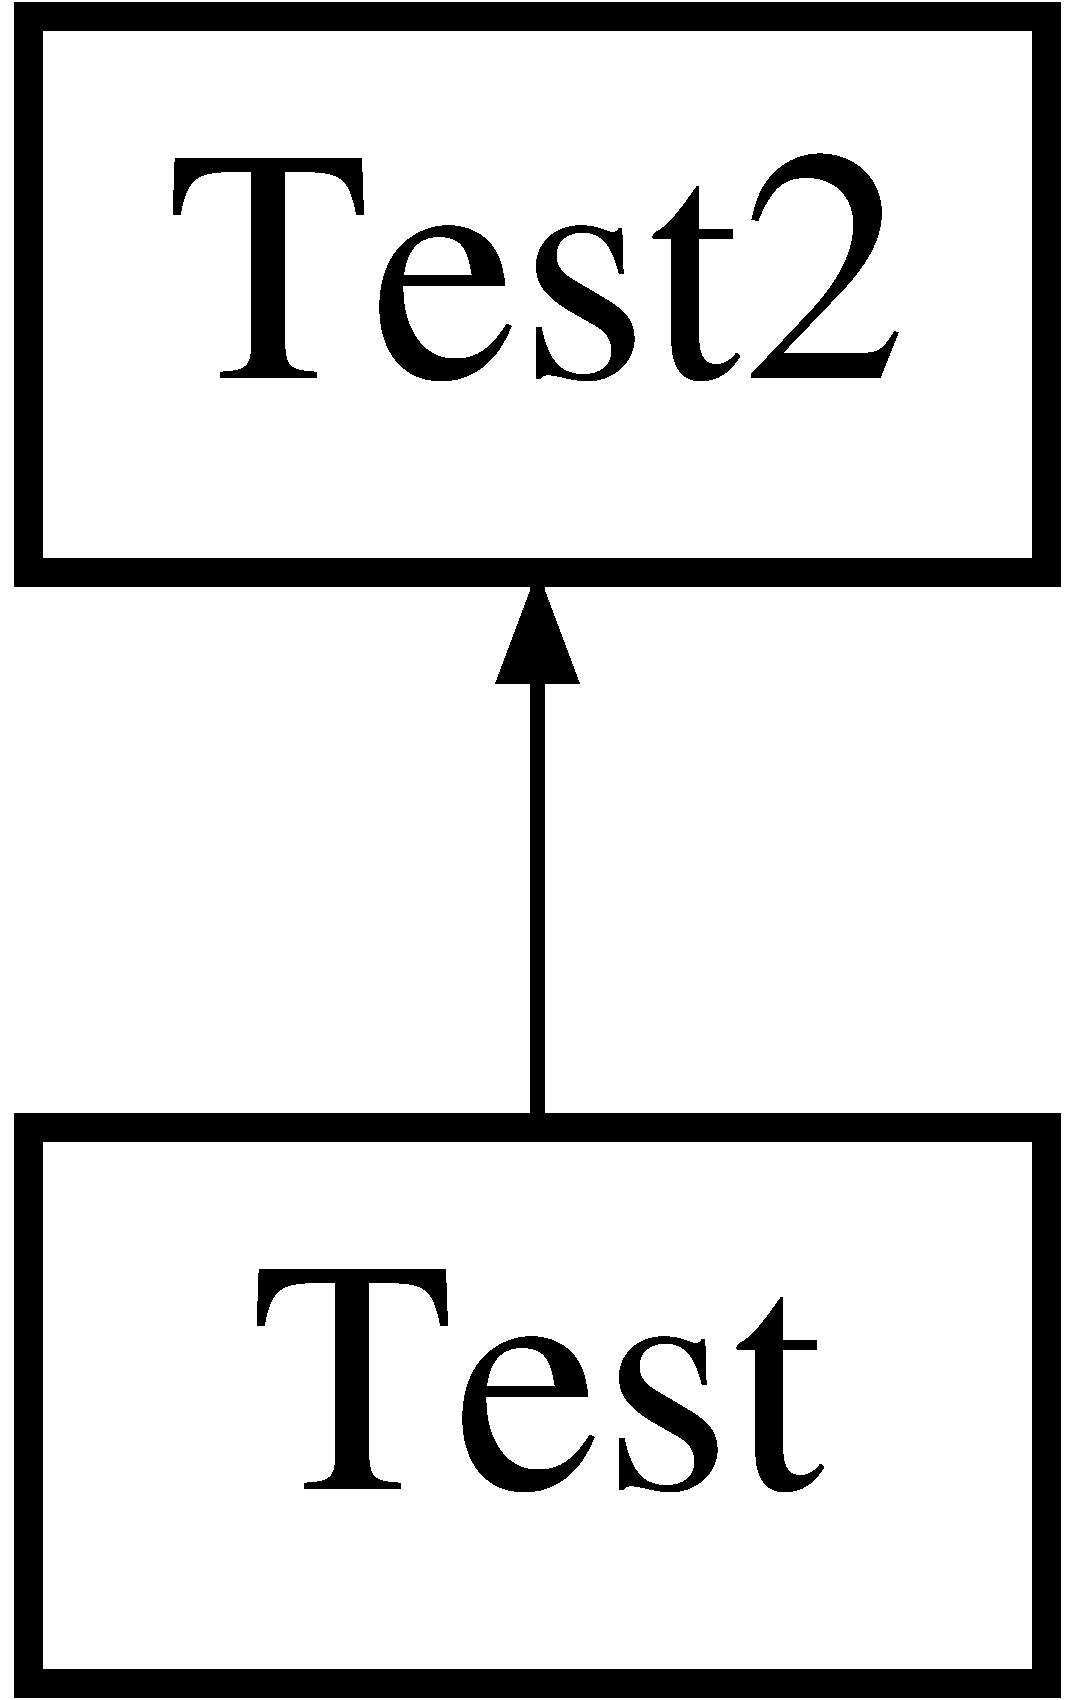
\includegraphics[height=2.000000cm]{class_test}
\end{center}
\end{figure}
\subsection*{Public Member Functions}
\begin{DoxyCompactItemize}
\item 
\hypertarget{class_test_a464592a38148f81120d99e66571cdcc4}{}{\bfseries testfunc} ()\label{class_test_a464592a38148f81120d99e66571cdcc4}

\end{DoxyCompactItemize}
\subsection*{Data Fields}
\begin{DoxyCompactItemize}
\item 
\hypertarget{class_test_aeb0df635d20f25c3f9de66ebc01b57e1}{}\hyperlink{class_test_aeb0df635d20f25c3f9de66ebc01b57e1}{\$member\+\_\+public} = \textquotesingle{}adsf\textquotesingle{}\label{class_test_aeb0df635d20f25c3f9de66ebc01b57e1}

\begin{DoxyCompactList}\small\item\em Public member of the \hyperlink{class_test}{Test} class. \end{DoxyCompactList}\end{DoxyCompactItemize}
\subsection*{Protected Attributes}
\begin{DoxyCompactItemize}
\item 
\hypertarget{class_test_aebac60379e54f5cd332b8bdcd4736412}{}\hyperlink{class_test_aebac60379e54f5cd332b8bdcd4736412}{\$member\+\_\+protected} = \mbox{[}\textquotesingle{}asdf\textquotesingle{}, \textquotesingle{}sadf\textquotesingle{}, \textquotesingle{}asdf\textquotesingle{}, \textquotesingle{}asdf\textquotesingle{}\mbox{]}\label{class_test_aebac60379e54f5cd332b8bdcd4736412}

\begin{DoxyCompactList}\small\item\em Protected member of the \hyperlink{class_test}{Test} class. \end{DoxyCompactList}\end{DoxyCompactItemize}


\subsection{Detailed Description}
Brief description. 

This is a detailed description of the class. 

The documentation for this class was generated from the following file\+:\begin{DoxyCompactItemize}
\item 
test.\+php\end{DoxyCompactItemize}

\chapter{File Documentation}
\hypertarget{test_8js}{}\section{test.\+js File Reference}
\label{test_8js}\index{test.\+js@{test.\+js}}


File for \hyperlink{class_test}{Test} function.  


\subsection*{Functions}
\begin{DoxyCompactItemize}
\item 
function \hyperlink{test_8js_a6585e56a8facf7d7f8c9dfeaf2ee3b89}{test} (param)
\end{DoxyCompactItemize}


\subsection{Detailed Description}
File for \hyperlink{class_test}{Test} function. 

Detailed file description. 

\subsection{Function Documentation}
\hypertarget{test_8js_a6585e56a8facf7d7f8c9dfeaf2ee3b89}{}\index{test.\+js@{test.\+js}!test@{test}}
\index{test@{test}!test.\+js@{test.\+js}}
\subsubsection[{test}]{\setlength{\rightskip}{0pt plus 5cm}function test (
\begin{DoxyParamCaption}
\item[{}]{param}
\end{DoxyParamCaption}
)}\label{test_8js_a6585e56a8facf7d7f8c9dfeaf2ee3b89}
Alerts string. This function alerts the string \char`\"{}test\char`\"{}. 
\begin{DoxyParams}{Parameters}
{\em \{\+String\}} & param Dummy parameter.\\
\hline
\end{DoxyParams}

%--- End generated contents ---

% Index
\backmatter
\newpage
\phantomsection
\clearemptydoublepage
\addcontentsline{toc}{chapter}{Index}
\printindex

\end{document}
